\section{算法}

\begin{frame}
  \begin{figure}  
  \centering
  \begin{tikzpicture}
    The graphic
    \node at (0,0)[fill=red!20,draw,starburst,drop shadow,text width=0.5cm]{
      两种算法的比较
    };
    \pause
    \node at (1.5,1.5) [right,fill=blue!20,draw,rectangle,rounded corners=3mm,text width=4cm]{
\begin{lstlisting}[mathescape=true]
int i,sum=0,n=100;
for (i=1;i<=n;i++)
  sum=sum+i;
printf("%d",sum);
\end{lstlisting}
};
    \node at (1.5,-1.5) [right,fill=blue!20,draw,rectangle,rounded corners=3mm,text width=4cm]{
\begin{lstlisting}[mathescape=true]
int i,sum=0,n=100;
sum=(n+1)*n/2;
printf("%d",sum);
      \end{lstlisting}
    };
  \end{tikzpicture}
  
\end{figure}


    
\end{frame}

\begin{frame}
  \begin{figure}  
  \centering
  \begin{tikzpicture}
    The graphic
    \node at (0,0)[fill=blue!20,draw,starburst,drop shadow,text width=7cm]{
      \blue{\large 算法}\\
      算法是解决特定问题求解步骤的描述,在计算机中表现为指令的有限序列,并且每条指令表示一个或多个操作.
    };

  \end{tikzpicture}
  
\end{figure}


 
  \pause 
  \begin{figure}
    \includegraphics[width=1in]{Chapters/Ch01/Fig/Hualazimi}
    \caption{阿勒.花剌子密(约780~约850,波斯数学家)}
  \end{figure}
\end{frame}

\begin{frame}
  \documentclass{article}
\usepackage{CJK} 
\usepackage{graphics}
\usepackage{pgf}
\usepackage{tikz}
\usetikzlibrary{calc,shadows}
\usetikzlibrary{decorations.markings,scopes}
\usetikzlibrary{arrows,snakes,backgrounds,shapes}
\usetikzlibrary{decorations.pathmorphing}
\usepackage{listings}
\renewcommand{\ttdefault}{pcr}
\lstset{
  keywordstyle=\color{blue!70},
  frame=single,
  basicstyle=\ttfamily\bfseries\small,
  commentstyle=\small\color{red},
  rulesepcolor=\color{red!20!green!20!blue!20},
  tabsize=4,
  numbersep=5pt,
  %% backgroundcolor=\color{black!10},
  showspaces=false,
  showtabs=false,
  extendedchars=false,
  escapeinside=``,
  frame=no
}

\newcommand{\blue}{\textcolor{blue}}
\newcommand{\red}{\textcolor{red}}
\newcommand{\purple}{\textcolor{purple}}


\pgfrealjobname{survey}
\begin{document}
\begin{CJK}{UTF8}{gkai} 
  \beginpgfgraphicnamed{AlgProp}
  \begin{tikzpicture}
    The graphic
    \node at (0,0)[fill=blue!20,draw,starburst,drop shadow,text width=0.8cm]{
      算法特性
    };

    \node at (0,2) [right,fill=red!20,draw,rectangle callout,callout relative pointer={(-0.6,-0.5)},rounded corners=3mm,text width=3cm]{
      \blue{输入}\\
      有零个或多个输入
    };
    \node at (2,0.8) [right,fill=red!20,draw,ellipse callout,callout relative pointer={(-1.4,-0.3)},text width=3.6cm]{
      \blue{输出}\\
      至少有一个或多个输出
    };
    \node at (2,-1) [right,fill=red!20,draw,rectangle callout,callout relative pointer={(-1,0.1)},rounded corners=3mm,text width=5cm]{
      \blue{有穷性}\\
      在执行有限步后,会自动结束而不出现无限循环,并且每一步在可接受的时间内完成
    };

    \node at (1,-3.5) [right,fill=red!20,draw,ellipse callout,callout relative pointer={(-2.2,1.5)},text width=4cm]{
      \blue{确定性}\\
      每一步都有确定的含义,不出现二义性
    };
    \node at (-2,-3) [right,fill=red!20,draw,rectangle callout,callout relative pointer={(0.3,0.7)},rounded corners=3mm,text width=2.5cm]{
      \blue{可行性}\\
      每一步都必须可行,能通过执行有限次数完成
    };
  \end{tikzpicture}
  \endpgfgraphicnamed  
\end{CJK}

\end{document}


    
  
\end{frame}


\begin{frame}
  \documentclass{article}
\usepackage{CJK} 
\usepackage{graphics}
\usepackage{pgf}
\usepackage{tikz}
\usetikzlibrary{calc,shadows}
\usetikzlibrary{decorations.markings,scopes}
\usetikzlibrary{arrows,snakes,backgrounds,shapes}
\usetikzlibrary{decorations.pathmorphing}
\usepackage{listings}
\renewcommand{\ttdefault}{pcr}
\lstset{
  keywordstyle=\color{blue!70},
  frame=single,
  basicstyle=\ttfamily\bfseries\small,
  commentstyle=\small\color{red},
  rulesepcolor=\color{red!20!green!20!blue!20},
  tabsize=4,
  numbersep=5pt,
  %% backgroundcolor=\color{black!10},
  showspaces=false,
  showtabs=false,
  extendedchars=false,
  escapeinside=``,
  frame=no
}

\newcommand{\blue}{\textcolor{blue}}
\newcommand{\red}{\textcolor{red}}
\newcommand{\purple}{\textcolor{purple}}


\pgfrealjobname{survey}
\begin{document}
\begin{CJK}{UTF8}{gkai} 
  \beginpgfgraphicnamed{AlgDesign}
  \begin{tikzpicture}
    The graphic
    \node at (0,0)[fill=blue!20,draw,starburst,drop shadow,text width=0.8cm]{
      算法设计要求
    };
    %% \node at (0,2) [right,fill=red!20,draw,rectangle callout,callout relative pointer={(-0.6,-0.5)},rounded corners=3mm,text width=3cm]{ 
    \node at (1.5,0) [right,fill=red!20,draw,rectangle split, rectangle split parts=4,rounded corners=3mm,text width=7cm]{
      \blue{正确性}\\
      算法至少应该具有输入、输出和加工处理无歧义性,能正确反映问题的需求、能得到问题的正确答案。
      \begin{itemize}
      \item 无语法错误
      \item 对合法输入能产生满足要求的输出
      \item 对非法输入能给出满足规格的说明
      \item 对精心选择的甚至是刁难的测试数据都有满足要求的输出
      \end{itemize}
      \nodepart{second}
      \blue{可读性}\\
      便于阅读、理解和交流
      \nodepart{third}
      \blue{健壮性}\\
      当输入不合法时,也能做出相应处理,而不是产生异常或莫名其妙的结果
      \nodepart{fourth}
      \blue{时间效率高和存储量低}
    };   
  \end{tikzpicture}
  \endpgfgraphicnamed  
\end{CJK}

\end{document}


    
  
\end{frame}

\begin{frame}
  \begin{figure}
  
  \centering
    \begin{tikzpicture}
    The graphic
    \node at (0,0)[fill=blue!20,draw,starburst,drop shadow,text width=0.8cm]{
      算法效率度量方法
    };
    \pause 
    %% \node at (0,2) [right,fill=red!20,draw,rectangle callout,callout relative pointer={(-0.6,-0.5)},rounded corners=3mm,text width=3cm]{ 
    \node at (2,1) [right,fill=red!20,draw,ellipse callout,callout relative pointer={(-0.8,-0.1)},text width=3cm]{
      \blue{事后统计方法}
    };
    \pause 
    \node at (2,-1) [right,fill=red!20,draw,ellipse callout,callout relative pointer={(-0.8,0.1)},text width=3cm]{
      \blue{事前分析估算方法}
    };

  \end{tikzpicture}
\end{figure}
    
  
\end{frame}

\begin{frame}
  \documentclass{article}
\usepackage{CJK} 
\usepackage{graphics}
\usepackage{pgf}
\usepackage{tikz}
\usetikzlibrary{calc,shadows}
\usetikzlibrary{decorations.markings,scopes}
\usetikzlibrary{arrows,snakes,backgrounds,shapes}
\usetikzlibrary{decorations.pathmorphing}
\usepackage{listings}
\renewcommand{\ttdefault}{pcr}
\lstset{
  keywordstyle=\color{blue!70},
  frame=single,
  basicstyle=\ttfamily\bfseries\small,
  commentstyle=\small\color{red},
  rulesepcolor=\color{red!20!green!20!blue!20},
  tabsize=4,
  numbersep=5pt,
  %% backgroundcolor=\color{black!10},
  showspaces=false,
  showtabs=false,
  extendedchars=false,
  escapeinside=``,
  frame=no
}

\newcommand{\blue}{\textcolor{blue}}
\newcommand{\red}{\textcolor{red}}
\newcommand{\purple}{\textcolor{purple}}


\pgfrealjobname{survey}
\begin{document}
\begin{CJK}{UTF8}{gkai} 
  \beginpgfgraphicnamed{AlgEffAfter}
  \begin{tikzpicture}[node distance=4.5cm]
    \node [fill=blue!20,draw,starburst,drop shadow,text width=7.5cm] (1) {
      \blue{\large 事后统计方法}\\
      通过设计好的测试程序和数据,利用计算机计时器对不同算法编制的程序的运行时间进行比较,从而确定效率的高低。
    };

    \node[below of=1,rectangle split,rectangle split parts=4,rounded corners=3mm,draw,text width=10cm,fill=red!20] {
      \blue{缺点}
      \nodepart{second}
      须依据算法事先编制好程序
      \nodepart{third}
      时间的比较依赖于软硬件等环境因素\\
      \begin{itemize}
      \item 不同性能的机器上算法的表现不尽相同;
      \item 不同操作系统、编译器等也会影响算法的运行结果;\\
      \item CPU使用率和内存占用情况也会造成微小差异。
      \end{itemize}
      \nodepart{fourth}
      测试数据设计困难,且程序运行时间还与测试数据的规模有很大关系,
      效率高的算法在小的测试数据面前往往得不到体现。
    };

  \end{tikzpicture}
  \endpgfgraphicnamed  
\end{CJK}

\end{document}


    
  
\end{frame}

\begin{frame}
  \begin{figure}
  
  \centering
    \begin{tikzpicture}[node distance=6cm]
  \node [fill=blue!20,draw,starburst,drop shadow,text width=5cm] (1) {
  \blue{\large 事前分析估算方法}\\
  在编制程序前,依据统计方法对算法进行估算。
  };
  \pause
  
  \node[below left of=1,rectangle split,rectangle split parts=5,rounded corners=3mm,draw,text width=7cm,fill=red!20] (2){
    \blue{程序运行时间取决于}
      \nodepart{two}
      (1)~算法采用的策略、方法 (\red{算法好坏的根本})
      \nodepart{three}
      (2)~编译产生的代码质量 (\red{软件支持})
      \nodepart{four}
      (3)~问题的输入规模 
      \nodepart{five}
      (4)~机器执行指令的速度 (\red{硬件性能})
    };
  \pause
    \node[right of=2,rectangle split,ellipse,draw,text width=2.5cm,fill=red!20] {
      程序的运行时间,依赖于算法的好坏和问题的输入规模。
    };

  \end{tikzpicture}

\end{figure}
    
  
\end{frame}

\begin{frame}
  \begin{figure}
  \centering
  \begin{tikzpicture}[node distance=2.5cm]

    \node[rectangle split,rectangle split parts=3,rounded corners=3mm,draw,text width=7cm,fill=red!20](1){
\begin{lstlisting}[language=C,mathescape]
for(i=1;i<=n;i++)
  sum+=i;          //`执行$n$次`
\end{lstlisting}
\nodepart{two}
\begin{lstlisting}[language=C]
sum=(n+1)*n/2;     //`执行$1$次`
\end{lstlisting}
\nodepart{three}
\begin{lstlisting}[language=C]
for(i=1;i<=n;i++)
  for(j=1;j<=n;j++){
    x++;           //`执行$n\times n$次`
    sum+=x;
  }
\end{lstlisting}
    };
    
  \end{tikzpicture}
\end{figure}


    
\end{frame}

\begin{frame}
  \begin{figure}
  
  \centering
  \begin{tikzpicture}[node distance=2.5cm]

    \begin{axis}[
        xmin=0, xmax=12,
        ymin=0, ymax=120,
        extra x ticks={2,4,6,8,10},
        extra y ticks={20,40,60,80,100},
        extra tick style={grid=major},
        ylabel=算法实际操作数量,
        xlabel=问题输入规模$n$,
        legend style={at={(1,0.5)},anchor=east}
      ]
      \addplot[domain=1:10,purple]{1};
      \addplot[domain=1:10,blue]{x};
      \addplot[domain=1:10,red]{x*x};
      \legend{$1$,$n$,$n^2$}
    \end{axis}
    
  \end{tikzpicture}
  
\end{figure}



    
  
\end{frame}

\begin{frame}
  \begin{figure}
  
  \centering
\begin{tikzpicture}[node distance=4.3cm]
  \node [fill=blue!20,draw,starburst,drop shadow,text width=6cm] (1) {
  \blue{\large 函数的渐近增长}\\
  给定两个函数$f(n)$和$g(n)$,若$\exists N \in \mathbb N$, s.t. $\forall n>N$, $f(n)$总是比$g(n)$大,
  我们就说$f(n)$的增长渐近快于$g(n)$.
  };
  \end{tikzpicture}
  
\end{figure}


    
  \pause 

  \begin{table}
    \begin{tabular}{|l|r|r|r|r|}\hline
      次数$n$&算法$A$&算法$A^\prime$&算法$B$&算法$B^\prime$\\
      & $(2n+3)$&$(2n)$&$(3n+1)$&$(3n)$\\\hline
      1  &  5&  2&  4&  3\\\hline
      2  &  7&  4&  7&  6\\\hline
      3  &  9&  6& 10&  9\\\hline
      10 & 23& 20& 31& 30\\\hline
      100&203&200&301&300\\\hline      
    \end{tabular}
  \end{table}
\end{frame}


\begin{frame}
  \begin{table}
    \begin{tabular}{|l|r|r|r|r|}\hline
      次数$n$&算法$C$&算法$C^\prime$&算法$D$&算法$D^\prime$\\
      & $(4n+8)$&$(n)$&$(2n^2+1)$&$(n^2)$\\\hline
      1   &   12&    1&        3&        2\\\hline
      2   &   16&    2&        9&        4\\\hline
      3   &   20&    3&       19&        9\\\hline
      10  &   48&   10&      201&      100\\\hline
      100 &  408&  100&   20 001&   10 000\\\hline
      1000&4 008&1 000&2 000 001&1 000 000\\\hline      
    \end{tabular}
  \end{table}
  \pause
  \begin{figure}
  
  \centering
  \begin{tikzpicture}
    \node at (1.5,1) [right,fill=red!20,draw,ellipse callout,callout relative pointer={(-0.8,0.2)},text width=5cm,text=blue]{
      函数的渐近增长可忽略加法常数,并且最高次项的系数也不重要。
    };
  \end{tikzpicture}
  
\end{figure}

    
  

\end{frame}


\begin{frame}
  \begin{table}
    \begin{tabular}{|l|r|r|r|r|}\hline
      次数$n$&算法$E$&算法$E^\prime$&算法$F$&算法$F^\prime$\\
      &$(2n^2+3n+1)$&$(n^2)$&$(2n^3+3n+1)$&$(n^3)$\\
      \hline
      1   &     6&     1&        6&        1\\\hline
      2   &    15&     4&       23&        8\\\hline
      3   &    28&     9&       64&       27\\\hline
      10  &   231&   100&    2 031&    1 000\\\hline
      100 &20 301&10 000&2 000 301&1 000 000\\\hline
    \end{tabular}
  \end{table}

  \pause
  \documentclass{article}
\usepackage{CJK} 
\usepackage{graphics}
\usepackage{pgf}
\usepackage{tikz}
\usetikzlibrary{calc,shadows}
\usetikzlibrary{decorations.markings,scopes}
\usetikzlibrary{arrows,snakes,backgrounds,shapes}
\usetikzlibrary{decorations.pathmorphing}
\usepackage{listings}
\renewcommand{\ttdefault}{pcr}
\lstset{
  keywordstyle=\color{blue!70},
  frame=single,
  basicstyle=\ttfamily\bfseries\small,
  commentstyle=\small\color{red},
  rulesepcolor=\color{red!20!green!20!blue!20},
  tabsize=4,
  numbersep=5pt,
  %% backgroundcolor=\color{black!10},
  showspaces=false,
  showtabs=false,
  extendedchars=false,
  escapeinside=``,
  frame=no
}

\newcommand{\blue}{\textcolor{blue}}
\newcommand{\red}{\textcolor{red}}
\newcommand{\purple}{\textcolor{purple}}


\pgfrealjobname{survey}
\begin{document}
\begin{CJK}{UTF8}{gkai} 
  \beginpgfgraphicnamed{FuncAymInc2}
  \begin{tikzpicture}
    \node at (1.5,1) [right,fill=red!20,draw,ellipse callout,callout relative pointer={(-0.8,0.2)},text width=5cm,text=blue]{
      最高次项的指数越大,随着$n$的增长,函数结果也会变得增长特别快。
    };
  \end{tikzpicture}
  \endpgfgraphicnamed  
\end{CJK}

\end{document}


    
  

\end{frame}


\begin{frame}
  \begin{table}
    \begin{tabular}{|l|r|r|r|r|}\hline
      次数$n$&算法$G$&算法$H$&算法$I$\\
            &$(2n^2)$&$(3n+1)$&$(2n^2+3n+1)$\\
      \hline
      1        &                2&        4&                 6\\\hline
      2        &                8&        7&                15\\\hline
      5        &               50&       16&                66\\\hline
      10       &              200&       31&               231\\\hline
      100      &           20 000&      301&            20 301\\\hline
      1,000    &        2 000 000&    3 001&         2 003 001\\\hline
      10,000   &      200 000 000&   30 001&       200 030 001\\\hline
      100,000  &   20 000 000 000&  300 001&    20 000 300 001\\\hline
      1,000,000&2 000 000 000 000&3 000 001& 2 000 003 000 001\\\hline
    \end{tabular}
  \end{table}
  \pause
  \begin{zhu}
    当$n$越来越大时,$3n+1$的结果与$2n^2$相比,几乎可以忽略不计。也就是说,随着$n$的不断增大,
    算法$G$其实很接近于算法$I$.
  \end{zhu}

\end{frame}


\begin{frame}


  \begin{figure}
  
  \centering
  \begin{tikzpicture}
    \node [fill=blue!20,draw,starburst,drop shadow,text width=6cm] (1) {
      判断一个算法的效率时,函数中的常数与其他次要项可以忽略,而更应该关注主项(最高阶项)的阶数。
    };
  \end{tikzpicture}
  
\end{figure}
    
  

\end{frame}


\begin{frame}
  \begin{figure}
  \centering
  \begin{tikzpicture}[node distance=4cm]
    \node [fill=blue!20,draw,starburst,drop shadow,text width=3.5cm,text=blue] (1) {
      {\large 算法时间复杂度}
    };
    \node [below of=1,fill=red!20,draw,rectangle,rounded corners=4mm,text width=7.8cm] (2) {
      在进行算法分析时,语句总的执行次数$T(n)$是关于问题规模$n$的函数,
      进而分析$T(n)$随$n$的变化情况并确定$T(n)$的数量级。算法的时间复杂度,也就是算法的时间量度,
      记作
      $$
      T(n)=O(f(n)).
      $$
      它表示随着$n$的增大,算法执行时间的增长率和$f(n)$的增长率相同,称为算法的渐近时间复杂度,
      简称为时间复杂度,其中$f(n)$是关于$n$的某个函数。
    };

    \pause 
    \node at (1.6,-3.5)[right,fill=green!20,draw,ellipse callout,callout relative pointer={(-0.8,-0.2)},text width=2cm,text=blue]{
      大O记法
    };
  \end{tikzpicture}
  
\end{figure}
    
\end{frame}

\begin{frame}
  \begin{figure}
  \centering
  \begin{tikzpicture}[node distance=3.2cm]
    \node [fill=blue!20,draw,starburst,drop shadow,text width=6cm,text=blue] (1) {
      如何分析一个算法的时间复杂度?即如何推导大O阶?
    };

    \pause 
    \node [below of=1,fill=red!20,draw,rectangle split,rectangle split parts=4,rounded corners=4mm,text width=8.5cm,text=blue]{
      1.~用常数1取代运行次数中的所有加法常数;
      \nodepart{two}
      2.~在修改后的运行次数函数中,只保留最高阶项;
      \nodepart{three}
      3.~如果最高阶项存在且不是1,则去除最高阶项的系数。
      \nodepart{four}
      得到的结果就是大O阶。
    };
  \end{tikzpicture}
  
\end{figure}
    
\end{frame}


\begin{frame}
  \begin{figure}
  \centering
  \begin{tikzpicture}[node distance=2cm]
    \node [fill=blue!20,draw,starburst,drop shadow,text width=2cm,text=blue] (1) {
      常数阶$O(1)$
    };

    \node [below of=1,fill=red!20,draw,rectangle,rounded corners=4mm,text width=8cm,text=blue]{
      \begin{lstlisting}[language=C]
int sum=0,n=100;  //`执行1次`
sum=(n+1)*n/2;    //`执行1次`
printf("%d",sum); //`执行1次`
      \end{lstlisting}
    };
  \end{tikzpicture}
\end{figure}

    
\end{frame}

\begin{frame}
  \begin{figure}
  \centering
  \begin{tikzpicture}[node distance=3cm]
    \node [fill=blue!20,draw,starburst,drop shadow,text width=2cm,text=blue] (1) {
      常数阶$O(1)$
    };

    \node [below of=1,fill=red!20,draw,rectangle,rounded corners=4mm,text width=8cm,text=blue]{
      \begin{lstlisting}[language=C]
int sum=0,n=100;  //`执行1次`
sum=(n+1)*n/2;    //`执行第1次`
sum=(n+1)*n/2;    //`执行第2次`
sum=(n+1)*n/2;    //`执行第3次`
sum=(n+1)*n/2;    //`执行第4次`
sum=(n+1)*n/2;    //`执行第5次`
printf("%d",sum); //`执行1次`
      \end{lstlisting}
    };
  \end{tikzpicture}
\end{figure}


    
\end{frame}


\begin{frame}
  \begin{figure}
  
  \centering

  \begin{tikzpicture}[node distance=3cm]
    \node [fill=blue!20,draw,starburst,drop shadow,text width=2cm,text=blue] (1) {
      线性阶$O(n)$
    };

    \node [below of=1,fill=red!20,draw,rectangle,rounded corners=4mm,text width=6cm,text=blue]{
      \begin{lstlisting}[language=C]
int i;
for (i=0;i<n;i++}
    //`时间复杂度为$O(1)$的语句块`
      \end{lstlisting}
    };
  \end{tikzpicture}
  
\end{figure}


    
  
\end{frame}

\begin{frame}
  \begin{figure}
  \centering
  \begin{tikzpicture}[node distance=2.8cm]
    \node [fill=blue!20,draw,starburst,drop shadow,text width=3cm,text=blue]
    (1) {
      对数阶$O(\log n)$
    };

    \node [below of=1,fill=red!20,draw,rectangle,rounded corners=4mm,text width=6cm,text=blue]
    (2) {
      \begin{lstlisting}[language=C,frame=no]
int count=1;
while (count<n){
  count*=2;
  //`时间复杂度为$O(1)$的语句块`
}
      \end{lstlisting}
    };
\pause 
    \node [below of=2,fill=green!40,draw,rectangle callout,callout relative pointer={(-0.5,1)},rounded corners=4mm,text width=8cm,text=blue]
    (3) {
      $$
      2^x=n ~\Longrightarrow ~
      x=\log_2 n 
      = \frac{\log n}{\log 2}.
      $$
    };
    
  \end{tikzpicture}
\end{figure}  


    
\end{frame}

\begin{frame}
  \begin{figure}
  \centering
  \begin{tikzpicture}[node distance=4.6cm]
    
    
    \node [fill=red!20,draw,rectangle split,rectangle split parts=3,rounded corners=4mm,text width=6cm,text=blue]
    (2){
      \begin{lstlisting}[language=C,frame=no]
int i,j;
for (i=0;i<n;i++)
  for (j=0;j<n;j++)
    //`时间复杂度为$O(1)$的语句块`
      \end{lstlisting}
      \nodepart{two}
      \begin{lstlisting}[language=C,frame=no]
int i,j;
for (i=0;i<m;i++)
  for (j=0;j<n;j++)
    //`时间复杂度为$O(1)$的语句块`
      \end{lstlisting}
      \nodepart{three}
      \begin{lstlisting}[language=C,frame=no]
int i,j;
for (i=0;i<n;i++)
  for (j=i;j<n;j++)
    //`时间复杂度为$O(1)$的语句块`
      \end{lstlisting}
    };

    \node at(5,4) [fill=blue!20,draw,starburst,drop shadow,text width=3cm,text=blue]
    (1) {
      平方阶$O(n^2)$
    };
    \pause 
    \node at (4.8,2.2)[fill=green!40,draw,ellipse callout,callout relative pointer={(-1,0.5)},text width=1cm,text=blue]
    (3) {
      $O(n^2)$
    };

    \pause 
    \node at (4.8,0)[fill=green!40,draw,ellipse callout,callout relative pointer={(-1,-0.5)},text width=2cm,text=blue]
    (4) {
      $O(m\times n)$
    };

    \pause 
    \node at (4.6,-2)[fill=green!40,draw,rectangle callout,callout relative pointer={(-0.7,-0.2)},rounded corners=3mm,text width=7.5cm,text=blue]
    (5) {
      因$f(n)=n+\cdots+2+1=\frac{n(n+1)}{2}=\frac{n^2}2+\frac n2$,
      故时间复杂度为$O(n^2)$.
    };


  \end{tikzpicture}
\end{figure}

    
\end{frame}

\begin{frame}
  \begin{figure}
  \centering
  \begin{tikzpicture}[node distance=4cm]
    \node [fill=red!20,draw,rectangle split,rectangle split parts=2,rounded corners=4mm,text width=6cm,text=blue]
    (1){
      \begin{lstlisting}[language=C,frame=no]
int i,j;        
for (i=0;i<n;i++)
  function(i);
      \end{lstlisting}
      \nodepart{two}
      \begin{lstlisting}[language=C,frame=no]
void function(int i){
  print("%d",i);
}
      \end{lstlisting}
    }; 
    \node [below right of=1,fill=orange!40,draw,ellipse callout,callout relative pointer={(-2,0.6)},text width=3.5cm,text=blue]
    (2) {
      请分析时间复杂度.
    };
    \pause 
    \node [below of=1,fill=green!40,draw,ellipse callout,callout relative pointer={(-0.7,1.8)},text width=1cm,text=blue]
    (2) {
      $O(n)$
    };

  \end{tikzpicture}
\end{figure}

\end{frame}

\begin{frame}
  \input{Chapters/Ch01/Tikz/AlgOrder2}
\end{frame}

\begin{frame}
  \begin{figure}
  \centering
  \begin{tikzpicture}[node distance=4cm]
    \node [fill=red!20,draw,rectangle,rounded corners=4mm,text width=10cm,text=blue]
    (1){
      \begin{lstlisting}[language=C,frame=no]
n++;                 //`执行次数为$1$`
function(n);         //`执行次数为$n$`
int i,j;  
for (i=0;i<n;i++)    //`执行次数为$n^2$`
  function(i);
for (i=0;i<n;i++)   //`执行次数为$n(n+1)/2$`
  for (j=i;j<n;j++)
    //`时间复杂度为$O(1)$的语句块`
      \end{lstlisting}
    }; 
    \node [below right of=1,fill=orange!40,draw,ellipse callout,callout relative pointer={(-2,0.6)},text width=3.5cm,text=blue]
    (2) {
      请分析时间复杂度.
    };
    \pause 
    \node [below of=1,fill=green!40,draw,rectangle callout,callout relative pointer={(-0.7,1.8)},rounded corners=3mm,text width=8.5cm,text=blue]
    (2) {
      执行次数$f(n)=1+n+n^2+\frac{n(n+1)}2=\frac32n^2+\frac32n+1$,
      故时间复杂度为$O(n^2)$.
    };

  \end{tikzpicture}
\end{figure}

\end{frame}


\begin{frame}
  \begin{table}
    \caption{常见时间复杂度}
    \begin{tabular}{l|l|l}\hline
      执行次数函数&阶&非正式术语\\\hline
      $12$&$O(1)$&常数阶\\[0.05in]
      $2n+3$&$O(n)$&线性阶\\[0.05in]
      $3n^2+2n+1$&$O(n^2)$&平方阶\\[0.05in]
      $5\log_2n+20$&$O(\log n)$&对数阶\\[0.05in]
      $2n+3n\log_2n+19$&$O(n\log n)$&$n\log n$阶\\[0.05in]
      $6n^3+2n^2+3n+4$&$O(n^3)$&立方阶\\[0.05in]
      $2^n$&$O(2^n)$&指数阶\\\hline
    \end{tabular}
  \end{table}
  \pause 
  \begin{figure}
    \centering
    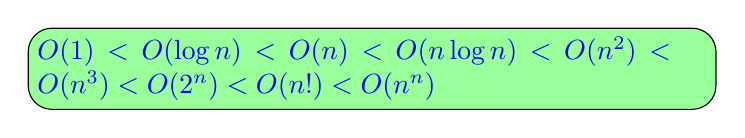
\begin{tikzpicture}
      \node [fill=green!40,draw,rectangle,rounded corners=3mm,text width=8.5cm,text=blue]
      (2) {
        $O(1)<O(\log n)<O(n)<O(n\log n)<O(n^2)<O(n^3)<O(2^n)<O(n!)<O(n^n)$
      };
    \end{tikzpicture}        
  \end{figure}
\end{frame}


\begin{frame}
  \begin{figure}
  \centering
  \begin{tikzpicture}[node distance=4cm]
    \node [fill=blue!20,draw,starburst,drop shadow,text width=2cm,text=blue] (1) {
      {\large 最坏情况}
    };
    \node [below left of=1,fill=red!20,draw,rectangle,rounded corners=4mm,text width=5.5cm] (2) {
      在$n$维随机数组中查找某个数字,
      \begin{itemize}
      \item 最好情况是出现在第一个位置,时间复杂度为$O(1)$;
      \item 最坏情况是出现在最后一个位置,时间复杂度为$O(n)$.
      \end{itemize}
    };

    \pause 
    \node at (3,-5)[text width=4.5cm,decorate,decoration=saw,fill=blue!20,draw,circle]{
      最坏情况运行时间是一种保证,亦即运行时间将不会再坏了。在应用中,这是一种最重要的需求,通常,除非特别指定,我们提到的运行时间都是最坏情况的运行时间。
    };
  \end{tikzpicture}
  
\end{figure}

\end{frame}

\begin{frame}
  \begin{figure}
  \centering
  \begin{tikzpicture}[node distance=4cm]
    \node [fill=blue!20,draw,starburst,drop shadow,text width=2cm,text=blue] (1) {
      {\large 平均情况}
    };
    \node [below left of=1,fill=red!20,draw,rectangle,rounded corners=4mm,text width=5.5cm] (2) {
      在$n$维随机数组中查找某个数字,
      \begin{itemize}
      \item 从概率角度讲,该数字在每个位置的可能性相同,故平均查找时间为$n/2$。
      \end{itemize}
    };

    \pause 
    \node at (3,-5)[text width=4.5cm,decorate,decoration=saw,fill=blue!20,draw,circle]{
      平均运行时间是所有情况中最有意义的,因为它是期望的运行时间。
    };
  \end{tikzpicture}
  
\end{figure}

\end{frame}

\begin{frame}
  \begin{figure}
  \centering
  \begin{tikzpicture}[node distance=3cm]
    \node [fill=blue!20,draw,starburst,drop shadow,text width=1cm,text=blue] (1) {
      {\large 小结}
    };
    \node [below of=1,fill=red!20,draw,rectangle,rounded corners=4mm,text width=9cm] (2) {
      对算法的分析,
      \begin{itemize}
      \item 一种方法是计算所有情况的平均值,这种时间复杂度的计算方法称为\blue{平均时间复杂度};
      \item 另一种是计算最坏情况下的时间复杂度,这种方法称为\blue{最坏时间复杂度}。
      \end{itemize}
      在没有特别说明的情况下,都指最坏时间复杂度。
    };

  \end{tikzpicture}
  
\end{figure}


\end{frame}

\begin{frame}
  \begin{figure}
  \centering
  \begin{tikzpicture}[node distance=4cm]
    \node [fill=blue!20,draw,starburst,drop shadow,text width=3.5cm,text=blue] (1) {
      {\large 算法空间复杂度}
    };
    \node [below of=1,fill=red!20,draw,rectangle,rounded corners=4mm,text width=7.8cm] (2) {
      通过计算算法所需的存储空间实现,其计算公式记作
      $$
      S(n)=O(f(n)).
      $$
      其中$n$为问题的规模,$f(n)$是语句关于$n$所占存储空间的函数。
    };
  \end{tikzpicture}
  
\end{figure}

\end{frame}

\begin{frame}
  \begin{figure}
  \centering
  \begin{tikzpicture}[node distance=0.8cm]
    \node at(0,0) [fill=blue!20,draw,starburst,drop shadow,text width=2cm,text=blue,text centered] (1) {
      {\large 总结回顾}
    };
    \pause 
    \node at(0,-1.5) [fill=red!20,draw,rectangle,rounded corners=2mm,text width=10cm,text centered] (2) {
      数据
    };
    \pause 
    \node [below of=2,fill=red!20,draw,rectangle,rounded corners=2mm,text width=10cm,text centered] (3) {
      数据对象
    };
    \pause 
    \node [below of=3,fill=red!20,draw,rectangle split,rectangle split parts=4,rectangle split horizontal,
      rounded corners=2mm,text width=2.3cm,text centered] (4) {
      数据元素 \nodepart{two}
      数据元素 \nodepart{three}
      数据元素 \nodepart{four}
      数据元素 
    };
    \pause 
    \node [below of=4,fill=red!20,draw,rectangle split,rectangle split parts=8,rectangle split horizontal,
      rounded corners=2mm,text width=1cm,text centered] (4) {
      \scriptsize{数据项1} \nodepart{two}
      \scriptsize{数据项2} \nodepart{three}
      \scriptsize{数据项1} \nodepart{four}
      \scriptsize{数据项2} \nodepart{five}
      \scriptsize{数据项1} \nodepart{six}
      \scriptsize{数据项2} \nodepart{seven}
      \scriptsize{数据项1} \nodepart{eight}
      \scriptsize{数据项2} 
    }; \pause 
    \node at (0,-6) [fill=green!40,draw,ellipse,rounded corners=2mm,text width=6cm,text centered]{
      数据结构是相互之间存在一种或多种特定关系的数据元素的集合。
    };

  \end{tikzpicture}
  
\end{figure}




\end{frame}

\begin{frame}
  \begin{figure}
  \centering
  \begin{tikzpicture}[node distance=4cm]
    \node at(0,0) [fill=blue!20,draw,starburst,drop shadow,text width=2cm,text=blue,text centered] (1) {
      {\large 总结回顾}
    };
    \pause     
    \node[below left of=1,fill=green!20,draw,rectangle split,rectangle split parts=5,rounded corners=2mm,text width=4cm,text centered,text=blue] (2) {
      \red{逻辑结构} \nodepart{two}
      集合结构 \nodepart{three}
      线性结构 \nodepart{four}
      树形结构 \nodepart{five}
      图形结构 
    };
    \pause 
    \node[below right of=1,fill=green!20,draw,rectangle split,rectangle split parts=3,rounded corners=2mm,text width=4cm,text centered,text=blue] (2) {
      \red{物理结构} \nodepart{two}
      顺序存储结构 \nodepart{three}
      链式存储结构 
    };
  \end{tikzpicture}
  
\end{figure}




\end{frame}

\begin{frame}
  \begin{figure}
  \centering
  \begin{tikzpicture}[node distance=2cm]
    \node at(0,0) [fill=blue!20,draw,starburst,drop shadow,text width=2cm,text=blue,text centered] (1) {
      {\large 总结回顾}
    };
    \pause     
    \node[below of=1,fill=green!20,draw,ellipse,text width=7.5cm,text=blue] (2) {
      \red{算法定义}:解决特定问题求解步骤的描述,在计算机中为指令的有限序列,且每条指令表示一个或多个操作。
    };
    \pause 
    \node[below of=2,fill=green!20,draw,ellipse,text width=7.5cm,text=blue] (3) {
      \red{算法特性}:有穷性、确定性、可行性、输入、输出
    };
    \pause 
    \node[below of=3,fill=green!20,draw,ellipse,text width=7.5cm,text=blue] (4) {
      \red{算法设计要求}:正确性、可读性、健壮性、高效率和低存储。
    };
  \end{tikzpicture}
  
\end{figure}




\end{frame}

\begin{frame}
  \begin{figure}
  \centering
  \begin{tikzpicture}[node distance=3cm]
    \node at(0,0) [fill=blue!20,draw,starburst,drop shadow,text width=2cm,text=blue,text centered] (1) {
      {\large 总结回顾}
    };
    \pause     
    \node[below of=1,fill=green!20,draw,ellipse,text width=7.5cm,text=blue] (2) {
      \red{算法度量方法}:事后统计方法(不科学、不准确)、事前分析估算方法。
    };
    \pause 
    \node[below of=2,fill=green!20,draw,ellipse,text width=7.5cm,text=blue] (3) {
      \red{函数的渐近增长}:  给定两个函数$f(n)$和$g(n)$,若$\exists N \in \mathbb N$, s.t. $\forall n>N$, $f(n)$总是比$g(n)$大,
      我们就说$f(n)$的增长渐近快于$g(n)$.
    };
  \end{tikzpicture}
  
\end{figure}




\end{frame}

\begin{frame}
  \begin{figure}
  \centering
  \begin{tikzpicture}[node distance=4cm]
    \node at(0,0) [fill=blue!20,draw,starburst,drop shadow,text width=2cm,text=blue,text centered] (1) {
      {\large 总结回顾}
    };
    \pause     
    \node[below of=1,fill=green!20,draw,ellipse,text width=8cm,text=blue] (3) {
      \red{大$O$阶推导过程}\\
      \begin{enumerate}[(1)]
      \item 用常数1取代运行次数中的所有加法常数;
      \item 在修改后的运行次数函数中,只保留最高阶项;
      \item 如果最高阶项存在且不是1,则去除最高阶项的系数。
      \end{enumerate}
      得到的结果就是大O阶。
    };
  \end{tikzpicture}
  
\end{figure}




\end{frame}


\begin{frame}
  \begin{figure}
  \centering
  \begin{tikzpicture}[node distance=2cm]
    \node at(0,0) [fill=blue!20,draw,starburst,drop shadow,text width=2cm,text=blue,text centered] (1) {
      {\large 总结回顾}
    };

    \pause 
    \node[below of=1,fill=green!20,draw,ellipse,text width=8cm,text=blue] (2) {
      $O(1)<O(\log n)<O(n)<O(n\log n)<O(n^2)<O(n^3)<O(2^n)<O(n!)<O(n^n)$
    };
    \pause 
    \node[below of=2,fill=green!20,draw,ellipse,text width=8cm,text=blue] (3) {
      算法最坏情况和平均情况,以及空间复杂度的概念。
    };

  \end{tikzpicture}
  
\end{figure}




\end{frame}
